\chapter{Redundanzreduktion}
\label{kap:Redundanzreduktion}

Die Redundanzreduktion ist ein wesentlicher Bestandteil der Videokompression. Sie wird benutzt um sowohl Redundanzen in der Codierung, mittels Entropiecodierung, als auch temporale Redundanzen, mittels Motion Compensation, so gut wie möglich zu entfernen. Die daraus resultierende Reduzierung der Videodaten hat, in der Regel, keinen Einfluss auf die Qualität des vom Nutzer erkennbaren Bildes.

\section{Entropiecodierung}

Die Entropiecodierung ist eine verlustfreie Methode zur Kompression von Daten im Generellen. Sie findet also nicht exklusiv Anwendung in der Videokompression, bildet für sie jedoch trotzdem eine wichtige Grundlage.

Ein Video kann als Nachricht, d.h. als Folge von Zeichen betrachtet werden. Jedes Zeichen an der Stelle i, hat dabei einen Informationsgehalt h, der sich aus seiner Eintrittswahrscheinlichkeit wie folgt berechnet:
\begin{align*}
h(i) = log(\frac{1}{p(i)})
\end{align*}

Die Entropie H ist der mittlerer Informationsgehalt von einem Zeichen einer Nachricht.
Sie berechnet sich aus der Summe aller Informationsgehälter mit einer Gewichtung der Wahrscheinlichkeit des iten-Zeichens:
\begin{align*}
H = \sum_{i=1}^E p(i) * h(i)
\end{align*}

Da die Zeichen einer Nachricht in den meisten Fällen nicht alle mit der gleichen Wahrscheinlichkeit auftreten, ist es sinnvoll die Codierung an die Wahrscheinlichkeiten der Auftretenden Zeichen anzupassen, sodass die am häufigst auftretenden Zeichen den jeweils kürzest möglichen Code erhalten.\cite{symes_peter_digital_2004}
Die mittlere Wortlänge L berechnet sich aus der Summe aller Codelängen mit einer Gewichtung der Wahrscheinlichkeit des iten-Zeichens: 
\begin{align*}
L = \sum_{i=1}^E p(i) * l(i)
\end{align*}


Das Shannon'sche Codierungstheorem besagt, dass, bei effizientes möglicher Kodierung mit eindeutiger Dekodierung, die mittlere Wortlänge eines Codes immer mindestens der Entropie einer Nachricht entsprechen muss. Dies bildet ein theoretisches Limit, dem sich so nah wie möglich angenähert werden soll.

Die Redundanz des Codes berechnet sich aus der Differenz von Entropie und mittlerer Wortlänge. Das Ziel für die Kompression eines Videos ist es, so wenig Code-Redundanz wie möglich zu erreichen, was nur durch Codes mit variabler Wortlänge zu erreichen ist.


\section{Motion Compensation}

Alle bis jetzt vorgestellten Ansätze der Videokompression beschäftigen sich mit der Kompression von Einzelbildern innerhalb eines Videos. Bei der Motion Compensation hingegen wird das Kompressionspotential ausgenutzt, dass innerhalb der Abhängigkeiten der Einzelbilder in einem Video steckt.
Videos bestehen meist aus zusammenhängenden Szenen mit größtenteils unverändertem Inhalt innerhalb einer jeweils solchen Szene, den sogenannten temporalen Redundanzen.

Man stelle sich zum Beispiel die folgende Szene vor: Eine Kamera filmt einen Mensch, unseren Protagonisten, der eine Straße entlang läuft und schließlich eine Bar betritt, eine typische Szene in Serien heutzutage.

Teilt man diese Szene in ihre Einzelbilder (Frames) auf, stellt man schnell fest, dass die Einzige Bewegung vom laufenden Protagonisten ausgeht und große Teile des Hintergrunds dabei in mehreren Bildern wiederholt werden.
Motion Compensation nutzt die Redundanz des Hintergrunds aus, indem es mehrfach vorhandene Teile jeweils nur ein Mal speichert und in den folgenden Bildern darauf referenziert um ein für den Zuschauer unverändertes Bild anzuzeigen.
Da Videos üblicherweise zum Großteil mit redundanten Bildteilen in einzelnen Szenen gefüllt sind, macht die von Motion Compensation erzielbare Kompression einen großen Teil des gesamt möglichen Kompressionpotentials innerhalb von Videos aus.

Damit Motion Compensation überhaupt funktionieren kann ist eine Aufteilung und Auswertung aller Video Einzelbilder in verschiedene Frames nötig.
\subsection{Frames}
Mit dem Kodieren teilt man alle Frames in eine bestimmte Bildart ein:
Es gibt rein intracodierte Frames, die sogenannten intracoded Frames (kurz I-Frames). Bei ihnen handelt es sich um einzelne Vollbilder, die von keinem anderen Bild des Videos abhängen. I-Frames sind also für sich stehende JPEG Bilder, welche mit den üblichen Methoden der Bildkompression verkleinert wurde, somit bieten diese die geringsten Kompression.
Außerdem gibt es intercodierte Frames, die nur eine vorhergesagte Differenz des Inhaltes in Abhängigkeit zu einem vorherigen I-Frame haben, die sogenannten predictive Frames (kurz P-Frames).
Als letztes gibt es bipredictive Frames (kurz B-Frames), die sehr ähnlich zu P-Frames sind, jedoch in zwei Richtungen intercodiert wurden. Sie speichern nur die jeweils vorhergesagte Differenz des Inhaltes zum Vorherigen, sowie dem Nächsten I- oder P-Frame.
Ein P-Frame benötigt nur etwa 1/3 und ein B-Frame nur etwa 1/9 so viel Speicherplatz wie ein I-Frames. \textcolor{blue}{TODO: Genauere Angaben finden}
Um die Vorhersagung erreichen zu können wird eine Reihenfolge der Codierung gewählt, die ungleich der Anzeigereihenfolge ist, was den Prozess zunehmend komplexer macht.\cite{symes_peter_digital_2004}

Ein kompletter Szenenwechsel, also das Ändern des kompletten Bildes, ohne statische Zusammenhänge, muss dem Encoder immer mitgeteilt werden. Dieser muss dann einen neuen I-Frame codieren, auf dem die folgenden P- und B-Frames basieren. Dadurch wird die potentielle Gefahr einer starken Artefaktbildung vorgebeugt.

Wenn man diese Aufteilung jedoch jeweils nur einmal pro Szene anwenden würde, würden mehrere Probleme bei wahllosem Zugriff entstehen. Wenn der I-Frame einer Szene fehlt oder übersprungen wird, würden die Änderungen, die in den folgenden P- und B-Frames festgehalten wurden, auf den falschen I-Frame angewendet, sodass im Video starke Artefakte entstehen, wie man auf \textcolor{blue}{Abbildung im Anhang (todo)} erkennt. Beim Ausfall eines P-Frames einer Szene würde grundsätzlich das Gleiche gleiche passieren, jedoch nur bei den noch folgenden P-Frames der Szene.

Um diese unschönen Artefakte beim Vor- und Zurückspulen zu verhindern, dürfte nur zu einem I-Frame gesprungen werden, welches bei einer Aufteilung pro Szene jeweils nur der Anfang einer neuen Szene wäre.

Da bei einem Großteil der Anwendungsfälle von Videos jedoch ein fast vollständig wahlfreier Zugriff gewünscht ist, teilt man jede Videosequenz in mehrere kleine aufeinanderfolgende Bildergruppen (Group of pictures, kurz GOP) auf. Eine GOP wird meist mit 2 Parametern angegeben, in diesem Beispiel N und M.
Dabei ist M eine bestimmte Anzahl von Frames aus denen die GOP besteht, also die Distanz von einem I-Frame zum nächsten I-Frame.
N gibt die Distanz von einem I- oder P-Frame, bis zum jeweils Nächsten an, somit ist N-1 die Anzahl von B-Frames, die nach einem I- oder P-Frame folgen.\cite{huszak2010analysing}
Eine Bildergruppe fängt immer mit einem I-Frame an und wiederholt sich bis zum Ende eines Videos mit einem konstanten Schema.

Mit den Parametern N=12 und M=4, würde die GOP dann aussehen wie folgt aussehen:
\begin{align*}
\bold{I\:BBB\:P\:BBB\:P\:BBB}
\end{align*}


Bei MPEG ist eine Aufteilung mit den Parametern M=3 bis 4 und N= 11 bis 15 üblich. \cite{symes_peter_digital_2004}

Betrachtet man ein Video mit einer üblichen Framerate von 25, dann ist dadurch wahlfreier Zugriff mit einer Genauigkeit von bis auf die Hälfte einer Sekunde gegeben. Außerdem wird der bei leichten Übertragungsfehlern auftretende Schaden minimiert, sodass das vom Endnutzer gesehene Video nur für sehr kurze Zeit Kompressionsartefakte aufweist, selbst bei komplettem Verlust eines I-Frames. 

\subsection{Makroblocks}

Beim Komprimieren eines Videos wird zunächst ein Frame pro GOP mittels Irrelevanzreduktion komprimiert und dann als Referenz zwischengespeichert. Die folgenden Bilder werden, um die vom Encoder benötigte Arbeit einfach aufteilen zu können, in sogenannte Makroblöcke unterteilt. Diese Makroblöcke sind bei den meisten Standards auf eine feste Größe von 16x16 Pixel gesetzt.\cite{symes_peter_digital_2004} Die neusten Standards wie h.246/AVC unterstützen hingegen variable Blockgrößen und mehrere Refernzbilder. \cite{lin2009vlsi}

\subsection{Motion Compensation}

Das in Makroblöcke aufgeteilte Bild wird vor der Durchführung der Irrelevanzreduktion mit der Referenz Block für Block verglichen um statische Bildinhalte zu 
erkennen. \cite{symes_peter_digital_2004} Ein Bildinhalt ist statisch, wenn sich ein Block von einem Bild zum nächsten nicht verändert hat. Alle statischen Bildinhalte werden dann entfernt, stattdessen wird auf den Inhalt der gespeicherten Referenz verwiesen. 
Damit sind zwar statische Bildinhalte kein Problem, allerdings kann, zum Beispiel bei einem Schwenken der Kamera, der trotzdem in beiden Bildern identisch vorhandene Hintergrund nicht kodiert werden, da sich sein Block in der Referenz zum Block des folgenden Bildes unterscheidet. Um diese immer noch redundanten Bildinformationen ebenfalls entfernen zu können, bedarf es einer komplexeren Vorgehensweise, der Motion Compensation.
Die Motion Compensation sucht jene Blöcke im neuem Frame mittels eines Block Matching Algorithmus heraus. Gefundene Blöcke werden mit einem Vektor, der von der Position des neuen Blocks, auf die Position des Ursprungsblocks aus der Referenz zeigt, kodiert.\cite{symes_peter_digital_2004} Beim Dekodieren kann dann mittels dieser Vektoren auf die Position des alten Blocks referenziert werden, sodass nur dieser Vektor gespeichert werden muss.
\begin{figure}[h!]
    \centering
    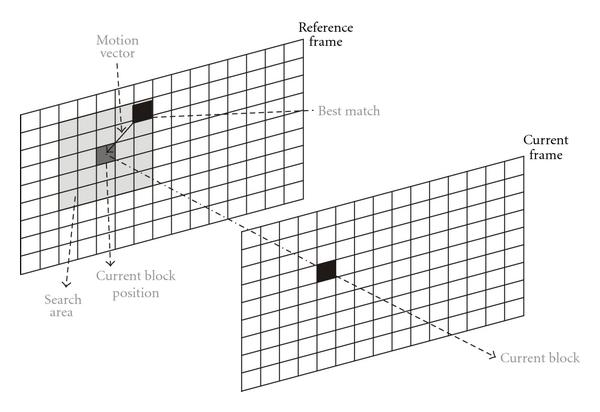
\includegraphics[scale=3]{images/3-2-3_motionCompensation.jpg}
    \caption{Suchen von identischen Blöcken in 2 Frames mittels Motion Compensation}
    \textit{Das Referenz Bild wird anschließend mit dem resultierenden Motion Vektor codiert}
    Quelle: \cite{lopes_memory_2012}
\end{figure}

%\subsection{Block Matching}

%TODO: Block matching mathematik erklären?

%\subsection{Probleme}
%Bei der Motion Compensation kann es zu Blockbildung bei vielen bewegenden Objekten %innerhalb einer Szene (Bsp: es schneit in einem Wald) kommen.
%\textcolor{blue}{Todo: Soll das hier noch hin? Zitat: VLSI Design for Video Coding S.%31-32} 